%% LyX 2.1.3 created this file.  For more info, see http://www.lyx.org/.
%% Do not edit unless you really know what you are doing.
\documentclass[english]{article}
\usepackage{ccfonts}
\usepackage[T1]{fontenc}
\usepackage[latin9]{inputenc}
\usepackage{geometry}
\geometry{verbose,tmargin=3cm,bmargin=3cm,lmargin=3cm,rmargin=3cm,headheight=3cm,headsep=3cm,footskip=3cm}
\setcounter{secnumdepth}{3}
\setcounter{tocdepth}{3}
\usepackage{url}
\usepackage{amsmath}
\usepackage{cancel}
\usepackage{graphicx}

\makeatletter
%%%%%%%%%%%%%%%%%%%%%%%%%%%%%% Textclass specific LaTeX commands.
\usepackage{beamerarticle,pgf}
% this default might be overridden by plain title style
\newcommand\makebeamertitle{\frame{\maketitle}}%
\AtBeginDocument{
\let\origtableofcontents=\tableofcontents
\def\tableofcontents{\@ifnextchar[{\origtableofcontents}{\gobbletableofcontents}}
\def\gobbletableofcontents#1{\origtableofcontents}
}

%%%%%%%%%%%%%%%%%%%%%%%%%%%%%% User specified LaTeX commands.
\usepackage{listings}
\usepackage{braket}

\makeatother

\usepackage{babel}
\begin{document}

\title{Measuring Geometric Phase using 3 Pin Holes :.}

\makebeamertitle
We describe a method a of measuring the geometric phase optically,
using 3 pin holes. This method is in stark contrast with conventional
methods where states are evolved and the relative phase measured after
completion of a cycle.


\section{Introduction}


\subsection{Geometric Phase}

Concept of geometric phase was discovered as a relative phase that
is introduced in an adiabatic and cyclic evolution of a state, between
the final and initial state. This relative phase has both the geometric
phase and what is known as the dynamic phase, which is the time integral
of the Hamiltonian. The concept since then, has been generalized to
work in cases of non-adiabatic evolution and then even to non-cyclic
evolution. 


\subsection{Conventional Measurement Scheme}

Experimentally, conventional measurement of the geometric phase is
associated with directly measuring the total phase difference between
the evolved and unevolved reference states. This requires phase calibration,
which is an experimental complication. Further, one must eliminate
the dynamic phase to obtain the geometric phase. 


\subsection{Kinematic Geometric Phase and the Proposed Scheme}

Direct observation of geometric phases using a three-pinhole interferometer
\textbf{PHYSICAL REVIEW A 81, 012104 (2010)}, \emph{Kobayashi et.
al.} propose a method of measurement of geometric phase, which is
built on the kinematic approach to geometric phase. In this approach,
the geometric phase is attributed to the structure of the Hilbert
space itself and doesn't require dynamics (evolution of states). One
can show that Geometric Phase is a ray space object and more explicitly,
it has been shown that for n points in the ray space, there exists
an entity known as the Bargmann invariant, from which the geometric
phase can be recovered. This geometric phase is that for a closed
curve obtained by connecting the n points with geodesics.

The proposed scheme involves use of 3 quantum states and letting them
interfere directly, viz. without evolving the system. From the intereferogram
thus obtained, using the 3 vertex Bargmann invariant and some more
details specific to the setup, it has been shown that the geometric
phase can be recovered. Further, since the initial 3 states are known,
one can theoretically evaluate the Geometric phase. Theory and experimental
observations have been shown to agree. Since this method doesn't require
evolution, the need for phase calibration and removal of dynamic phase
has been eliminated.


\section{Geometric Phase and Bargmann Invariant}

\begin{figure}
\begin{centering}

\includegraphics[width=8cm]{paperImages/1}
\par\end{centering}

\protect\caption{Schematic of the setup}


\end{figure}


As Figure 1 shows, three states $\ket{\psi_{j}}(j=1,2,3)$ represent
the internal states of the photon from three pinholes. The resultant
interferogram should and does contain three distinct interference
fringes due to each pinhole pair. To start with, superimpostion of
$\ket{\psi_{1}}$ and a $U(1)=e^{i\phi}$ shifted $\ket{\psi_{2}}$
leads to an intensity of 

\[
I\propto1+\left|\left\langle \psi_{1}|\psi_{2}\right\rangle \right|\cos\left(\phi+\arg\left\langle \psi_{1}|\psi_{2}\right\rangle \right)
\]
which can be derived easily as 
\[
\begin{aligned}\left|\psi\right\rangle  & =e^{i\phi}\left|\psi_{1}\right\rangle +\left|\psi_{2}\right\rangle \\
\left\langle \psi|\psi\right\rangle  & =\left(\left\langle \psi_{1}\right|e^{-i\phi}+\left\langle \psi_{2}\right|\right)\left(e^{i\phi}\left|\psi_{1}\right\rangle +\left|\psi_{2}\right\rangle \right)\\
 & =\left\langle \psi_{1}|\psi_{1}\right\rangle +\left\langle \psi_{2}|\psi_{2}\right\rangle +\left(e^{-i\phi}e^{i\text{arg}\left\langle \psi_{1}|\psi_{2}\right\rangle }\left|\left\langle \psi_{1}|\psi_{2}\right\rangle \right|+\text{hc}\right)\\
 & \propto1+\left|\left\langle \psi_{1}|\psi_{2}\right\rangle \right|\cos\left(\phi+\arg\left\langle \psi_{1}|\psi_{2}\right\rangle \right)
\end{aligned}
\]
Thus the interference fringes are shifted by the relative phase between
the states. In case of constructive interference, this phase is zero
and the states are called \emph{in phase}. Note however that this
property of the states is \emph{non transitive}. To make this explicit,
consider the following expression, which is manifestly invariant under
a local change of phases (gauge invariance).

\[
\begin{aligned}\Delta_{3}\left(\psi_{1},\psi_{2},\psi_{3}\right) & \equiv\left\langle \psi_{1}|\psi_{2}\right\rangle \left\langle \psi_{2}|\psi_{3}\right\rangle \left\langle \psi_{3}|\psi_{1}\right\rangle \\
 & =\text{tr}\left(\left|\psi_{2}\right\rangle \left\langle \psi_{2}|\psi_{3}\right\rangle \left\langle \psi_{3}|\psi_{1}\right\rangle \left\langle \psi_{1}\right|\right)\\
\implies\text{arg}\left(\Delta_{3}\left(\psi_{1},\psi_{2},\psi_{3}\right)\right) & =\arg\left(\left\langle \psi_{1}|\psi_{2}\right\rangle \left\langle \psi_{2}|\psi_{3}\right\rangle \left\langle \psi_{3}|\psi_{1}\right\rangle \right)\\
 & =\sum_{(i,j)\text{cycle}}\text{arg}\left\langle \psi_{j}|\psi_{j}\right\rangle 
\end{aligned}
\]
Here, if $\text{arg}\left\langle \psi_{1}|\psi_{2}\right\rangle =0$
and $\text{arg}\left\langle \psi_{2}|\psi_{3}\right\rangle =0$, that
is if the states 1 and 2 are in phase, 2 and 3 are in phase, then
$\text{arg}\left(\Delta_{3}\left(\psi_{1},\psi_{2},\psi_{3}\right)\right)=\text{arg}\left\langle \psi_{1}|\psi_{3}\right\rangle \ne0$
in general.

$\Delta_{3}$ is defined to be a 3 point \textbf{Bargmann Invariant}
and $\arg\Delta_{3}$, the \textbf{Pancharatnam Phase}. We recall/claim
that the Pancharatnam phase can be related to the geometric phase
corresponding to that of a triangle in the B space (or if you like,
that of a system whose trajectory is given by the triangle).\footnote{B `space' is a \emph{subset} of H (Hilbert Space) with $\left\langle \psi|\psi\right\rangle =1$.
Ray space is the subspace formed by $\rho_{\psi}=\ket{\psi}\bra{\psi}$
(idea is to remove the phase freedom)} This triangle has as vertices, the points corresponding to the 3
states. Its sides are formed by joining these points by geodesics.\footnote{Assuming an appropriately defined metric, this we had proved in the
course. It hinges on the fact that for a closed loop in B space, the
total phase is zero. In general $\phi_{\text{total}}=\phi_{\text{dyn}}+\phi_{\text{geom}}$
where for a geodesic between 2 points, $\phi_{\text{dyn}}=\text{arg}\left\langle \psi_{1}|\psi_{2}\right\rangle $.
With these assumptions and the fact that dynamic phase is additive,
the result stated should follow.} The relation is 
\[
\phi_{\text{goem}}=-\text{arg}\Delta_{3}\left(\psi_{1},\psi_{2},\psi_{3}\right)
\]
It can be further shown, that for a two state system (such as polarization
of photon, the case here), $\arg\Delta_{3}$ is proportional to the
solid angle ($\Omega$) of the spherical triangle on the Bloch sphere
with the three states as the vertices. 
\[
\phi_{\text{goem}}=-\frac{\Omega}{2}
\]



\section{Geometric Phase and Ridge Lines}

Consider again, the three pinholes irradiated with monochromatic light
of wavenumber $k$. Without any loss of generality, the location of
the three pinholes can be parametrized by $\mathbf{a}_{j}(j=1,2,3)$
such that $\left|\mathbf{a}_{j}\right|=a\,\forall\,j$, by simply
choosing the origin to be the circumcenter of the triangle. The source
plane is labeled to be at $z=0$. It is known that the state of a
photon can be expressed as a combination of a spatial part represented
by the spherical wave and the internal, polarization state part. The
state of photon from the $j^{th}$ pin-hole\footnote{If we assume that all the pinholes have the same probability of transmission},
on the observation plane $z=L$ is

\[
\left|\psi(\mathbf{r})\right\rangle =C\sum_{j=1}^{3}\frac{\text{exp}\left[i\left(k\left|\mathbf{R}-\mathbf{a}_{j}\right|+\phi_{j}\right)\right]}{\left|\mathbf{R}-\mathbf{a}_{j}\right|}\left|\psi_{j}\right\rangle 
\]
where $\mathbf{R}$ is the position vector on the observation plane
($z=L$); $\mathbf{r}\equiv\mathbf{R}-\left(\mathbf{R}.\mathbf{z}\right)\mathbf{z}$
(component of $\mathbf{R}$ perpendicular to $\mathbf{z}$, the unit
vector along z-axis); $C$ is dimensionless normalization; $\phi_{j}$
is the phase of $\left|\psi_{j}\right\rangle $ (the polarization
state of the $j^{th}$ source). If we make the para-axial approximation,
we get

\[
\begin{aligned}\mathbf{R}-\mathbf{a}_{j} & =\left(L\mathbf{z}+\mathbf{r}\right)-\mathbf{a}_{j}\\
\left|\mathbf{R}-\mathbf{a}_{j}\right| & =\left[\left(\left(L\mathbf{z}+\mathbf{r}\right)-\mathbf{a}_{j}\right)\left(\left(L\mathbf{z}+\mathbf{r}\right)-\mathbf{a}_{j}\right)\right]^{1/2}\\
 & =\left[\left(L\mathbf{z}+\mathbf{r}\right)\left(L\mathbf{z}+\mathbf{r}\right)-2\left(L\mathbf{z}+\mathbf{r}\right)\mathbf{a}_{j}+\mathbf{a}_{j}^{2}\right]^{1/2}\\
 & =\left[L^{2}+2L\cancelto{0}{\mathbf{z}.\mathbf{r}}+\mathbf{r}^{2}-2(L\cancelto{0}{\mathbf{z}.\mathbf{r}}+\mathbf{r}.\mathbf{a}_{j})+\mathbf{a}_{j}^{2}\right]^{1/2}\\
 & =\left[L^{2}+2\frac{r^{2}+a^{2}}{2}-2(\mathbf{r}.\mathbf{a}_{j})\right]^{1/2}\\
 & =L\left[1+2\left(\frac{r^{2}+a^{2}}{2L^{2}}-\frac{(\mathbf{r}.\mathbf{a}_{j})}{L^{2}}\right)\right]^{1/2}\\
 & \approx L\left[1+\frac{r^{2}+a^{2}}{2L^{2}}-\frac{(\mathbf{r}.\mathbf{a}_{j})}{L^{2}}\right]\\
 & =L+\frac{r^{2}+a^{2}}{2L}-\frac{(\mathbf{r}.\mathbf{a}_{j})}{L}
\end{aligned}
\]
\[
\left|\psi(\mathbf{r})\right\rangle \approx C\sum_{j=1}^{3}\frac{\text{exp}\left[i\left(k\left(L+\frac{r^{2}+a^{2}}{2L}-\frac{(\mathbf{r}.\mathbf{a}_{j})}{L}\right)+\phi_{j}\right)\right]}{L}\left|\psi_{j}\right\rangle 
\]
where we've used the fact that $\mathbf{a}_{j}^{2}=a^{2}$. In the
last step, in writing the denominator approximately as $L$, we have
also used a stronger condition, that is $\left|\mathbf{R}-\mathbf{a}_{j}\right|\ll\left(L^{3}/k\right)^{1/4}\ll L$.

The intensity distribution can then be written as 
\[
\begin{aligned}p(x,y) & =\left\langle \psi(\mathbf{r})|\psi(\mathbf{r})\right\rangle \\
 & =\frac{C^{2}}{L^{2}}\sum_{j,k=1}^{3}\text{exp}\left[-i\left(k\left(\cancel{L+\frac{r^{2}+a^{2}}{2L}}-\frac{(\mathbf{r}.\mathbf{a}_{j})}{L}\right)+\phi_{j}\right)\right]\text{exp}\left[i\left(k\left(\cancel{L+\frac{r^{2}+a^{2}}{2L}}-\frac{(\mathbf{r}.\mathbf{a}_{k})}{L}\right)+\phi_{k}\right)\right]\left\langle \psi_{j}|\psi_{k}\right\rangle \\
 & =\frac{C^{2}}{L^{2}}\left\{ 3+\sum_{j\neq k=1}^{3}\text{exp}\left[i\left(k\left(\frac{(\mathbf{r}.\mathbf{a}_{j})}{L}-\frac{(\mathbf{r}.\mathbf{a}_{k})}{L}\right)+\phi_{k}-\phi_{j}+\text{arg}\left\langle \psi_{j}|\psi_{k}\right\rangle \right)\right]\left|\left\langle \psi_{j}|\psi_{k}\right\rangle \right|\right\} \\
 & =\frac{C^{2}}{L^{2}}\left\{ 3+\sum_{\left(j,k\right)\text{cycle}}\cos\left[k\left(\frac{(\mathbf{r}.\mathbf{a}_{j})}{L}-\frac{(\mathbf{r}.\mathbf{a}_{k})}{L}\right)+\phi_{k}-\phi_{j}+\text{arg}\left\langle \psi_{j}|\psi_{k}\right\rangle \right]\left|\left\langle \psi_{j}|\psi_{k}\right\rangle \right|\right\} \\
 & =\frac{C^{2}}{L^{2}}\left\{ -3+\sum_{(i,j)\text{cycle}}P_{ij}(x,y)\right\} 
\end{aligned}
\]
which finally yields

\[
p(x,y)=\frac{C^{2}}{L^{2}}\left\{ -3+\sum_{(i,j)\text{cycle}}P_{ij}(x,y)\right\} 
\]
where 
\[
P_{ij}(x,y)\equiv2\left(1+\cos\left[(\mathbf{k}_{ij}.\mathbf{r})-\phi_{ij}+\text{arg}\left\langle \psi_{i}|\psi_{j}\right\rangle \right]\left|\left\langle \psi_{i}|\psi_{j}\right\rangle \right|\right)
\]
with $k_{ij}\equiv k(\mathbf{a}_{i}-\mathbf{a}_{j})/L$ and $\phi_{ij}\equiv\phi_{i}-\phi_{j}$.
This equation infact corresponds to that of the double slit interference
fringes between two states $\ket{\psi_{i}}$ and $\ket{\psi_{j}}$.
Thus, the three pin hole interferogram consists of sets of interference
fringes with distinct directions, given by $\mathbf{k}_{ij}$. Evidently,
the geometric phase information is contained in $P_{ij}$. To extract
this, we look at the condition for maximum intensity

\[
(\mathbf{k}_{ij}.\mathbf{r})-\phi_{ij}+\text{arg}\left\langle \psi_{i}|\psi_{j}\right\rangle =2n_{ij}\pi
\]
which is of the from $\mathbf{r}.\mathbf{k}=c$ (in 3d, this is a
plane, in 2d, its a line obviously) 
\[
\begin{aligned}(x\mathbf{x}+y\mathbf{y}).(k_{x}\mathbf{x}+k_{y}\mathbf{y}+k_{z}\mathbf{z}) & =c\\
 & =xk_{x}+yk_{y}
\end{aligned}
\]
Here $n_{ij}$ are integers. These equations define sets of three
distinct parallel lines which are called the \textbf{ridge lines}
on the observation plane. The area $S$ of the triangle formed by
these, called the \textbf{ridge triangle}. Using the formula for finding
the area of a triangle, given equations of the lines making the edges
as 
\[
\begin{aligned}a_{1}x+b_{1}y+c_{1} & =0\\
a_{2}x+b_{2}y+c_{2} & =0\\
a_{3}x+b_{3}y+c_{3} & =0
\end{aligned}
\]
is 
\[
\frac{\text{det}\left[\begin{array}{ccc}
a_{1} & b_{1} & c_{1}\\
a_{2} & b_{2} & c_{2}\\
a_{3} & b_{3} & c_{3}
\end{array}\right]^{2}}{2C_{1}C_{2}C_{3}}
\]
where $C_{i}=\text{cofactor of }c_{i}$, we finally obtain

\[
S=\frac{L^{2}}{4k^{2}S_{0}}\left\{ \text{arg}\left[\Delta_{3}\left(\psi_{1},\psi_{2},\psi_{3}\right)\right]-2n\pi\right\} ^{2}
\]
where $n=n_{12}+n_{23}+n_{31}$ and $S_{o}$ is the area of the triangle
of the three pinholes. 

Some points are wroth noting here. 
\begin{itemize}
\item The area of ridge triangle is related to $\arg\Delta_{3}$. We define
an \textbf{elemental ridge triangle}\emph{ }to be a ridge triangle
that encloses no ridge lines. For example, for $0\leq\arg\Delta_{3}<2\pi$
the ridge triangles with $n=0$ and $1$ are elemental. Clearly, the
$S$ with $n=0$ is proportional to square of geometric phase $\arg\Delta_{3}$;
for $n=1$ it is proportional to $2\pi-\arg\Delta_{3}$. 
\item Secondly, the gauge invariance of $\Delta_{3}$ carries over to the
area since by introducing a phase shift to one of pinholes, two sets
of ridge lines are displaced but the area is conserved. 
\item Third, the equation is proportional to the geometric phases regardless
of the vectors $\mathbf{a}_{i}$, thus essentially any geometry of
the three pinholes can form the ridge triangle. 
\end{itemize}

\section{Extraction of Ridge Lines}

In order to determine the ridge lines, rather than the straightforward
way of observing individual interference fringes $P_{ij}(x,y)$ by
closing one of the holes, we extract all the ridge lines in a single
shot from the combined interferogram $p(x,y)$. To start with, note
that for arbitrary $\mathbf{b},\,\mathbf{k}$ we have

\[
\begin{aligned}\mathbf{b}.\mathbf{\nabla}\left(\mathbf{k}.\mathbf{r}\right) & =b_{i}\frac{\partial}{\partial x_{i}}k_{j}r_{j}\\
 & =b_{i}k_{j}\left(\frac{\partial}{\partial x_{i}}r_{j}\right)\\
 & =b_{i}k_{j}\delta_{ij}\\
 & =\mathbf{b}.\mathbf{k}
\end{aligned}
\]
Now we define 
\[
\mathbf{b}_{i}\equiv\mathbf{e}_{z}\times(\mathbf{a}_{j}-\mathbf{a}_{k})=\frac{L}{k}\mathbf{e}_{z}\times\mathbf{k}_{jk}
\]
where $(i,j,k)=(1,2,3),(2,3,1),(3,1,2)$ NB: $\mathbf{b}_{i}\mathbf{k}_{jk}=0$.
Further note that the vector $b_{i}$ in $z=0$ is determined only
by the geometry of the three pinholes. If we consider the directional
derivative along $b_{i}$, since $b_{i}$ is orthogonal to $k_{jk}$
we can\footnote{The derivation is given below. This is just to motivate the approach.}
now eliminate one of the interference fringes $P_{ij}(x,y)$ from
the total interferogram $p(x,y)$ while the other fringes remain sinusoidal
functions. Another such directional derivative isolates the desired
oscillation term.

Let's explicitly derive this. Recall: $P_{ij}(x,y)\equiv2\left(1+\cos\left[(\mathbf{k}_{ij}.\mathbf{r})-\phi_{ij}+\text{arg}\left\langle \psi_{i}|\psi_{j}\right\rangle \right]\left|\left\langle \psi_{i}|\psi_{j}\right\rangle \right|\right)$.
Let's start with performing the first directional derivative.

\[
\begin{aligned}\left(\mathbf{b}_{1}.\nabla\right)p(x,y) & =\left(\mathbf{b}_{1}.\mathbf{\nabla}\right)\frac{C^{2}}{L^{2}}\left\{ -3+\sum_{(i,j)\text{cycle}}P_{ij}(x,y)\right\} \\
 & \propto\sum_{(i,k)\text{cycle}}\left(\mathbf{b}_{1}.\mathbf{\nabla}\right)P_{ik}(x,y)\\
 & \propto\sin\left[(\mathbf{k}_{12}.\mathbf{r})-\phi_{12}+\text{arg}\left\langle \psi_{1}|\psi_{2}\right\rangle \right]\left|\left\langle \psi_{1}|\psi_{2}\right\rangle \right|\cancelto{\mathbf{b}_{1}.\mathbf{k}_{12}}{\left(\mathbf{b}_{1}.\mathbf{\nabla}\right)(\mathbf{k}_{12}.\mathbf{r})}\\
 & +\sin\left[(\mathbf{k}_{23}.\mathbf{r})-\phi_{23}+\text{arg}\left\langle \psi_{2}|\psi_{3}\right\rangle \right]\left|\left\langle \psi_{2}|\psi_{3}\right\rangle \right|\cancelto{0}{\mathbf{b}_{1}.\mathbf{k}_{23}}\\
 & +\sin\left[(\mathbf{k}_{31}.\mathbf{r})-\phi_{31}+\text{arg}\left\langle \psi_{3}|\psi_{1}\right\rangle \right]\left|\left\langle \psi_{3}|\psi_{1}\right\rangle \right|\mathbf{b}_{1}.\mathbf{k}_{31}
\end{aligned}
\]
Now when it is applied again along $\mathbf{b}_{2}$, we get

\[
\begin{aligned}\left(\mathbf{b}_{2}.\nabla\right)\left(\mathbf{b}_{1}.\nabla\right)p(x,y) & \propto-\cos\left[(\mathbf{k}_{12}.\mathbf{r})-\phi_{12}+\text{arg}\left\langle \psi_{1}|\psi_{2}\right\rangle \right]\left|\left\langle \psi_{1}|\psi_{2}\right\rangle \right|\mathbf{b}_{1}.\mathbf{k}_{12}\mathbf{b}_{2}.\mathbf{k}_{12}\\
 & -\cos\left[(\mathbf{k}_{31}.\mathbf{r})-\phi_{31}+\text{arg}\left\langle \psi_{3}|\psi_{1}\right\rangle \right]\left|\left\langle \psi_{3}|\psi_{1}\right\rangle \right|\mathbf{b}_{1}.\mathbf{k}_{31}\cancelto{0}{\mathbf{b}_{2}.\mathbf{k}_{31}}\\
 & \propto\cos\left[(\mathbf{k}_{12}.\mathbf{r})-\phi_{12}+\text{arg}\left\langle \psi_{1}|\psi_{2}\right\rangle \right]\left|\left\langle \psi_{1}|\psi_{2}\right\rangle \right|
\end{aligned}
\]
which is precisely what we'd claimed to start with. NB: $\left(\mathbf{b}_{2}.\nabla\right)\left(\mathbf{b}_{1}.\nabla\right)p(x,y)=\left(\mathbf{b}_{1}.\nabla\right)\left(\mathbf{b}_{2}.\nabla\right)p(x,y)$

So in general then, I can write

\[
\left(\mathbf{b}_{i}.\mathbf{\nabla}\right)\left(\mathbf{b}_{j}.\mathbf{\nabla}\right)p(x,y)\propto\cos\left[(\mathbf{k}_{ij}.\mathbf{r})-\phi_{ij}+\text{arg}\left\langle \psi_{i}|\psi_{j}\right\rangle \right]\left|\left\langle \psi_{i}|\psi_{j}\right\rangle \right|
\]


Interferograms for the three pinholes are shown in Figure 3(a) and
the three sets of ridge lines thus extracted are shown in Figure 3(b).
Thus it is easy to determine the pure geometric phase instantaneously
as the square root of the area of the ridge triangle extracted directly
from the three pinhole interferogram for three arbitrary states. 


\section{Experiment}

For the experiment (Figure 2), a $532nm$ green laser source was used
for illuminating a thin copper foil that is perforated with three
$0.1mm$ radius pinholes. These pinholes lie on an equilateral triangle
of side $1.5mm$. The observation plane was placed at a distance of
approximately $2m$ from the pinholes, where the interfering patterns
were captured using a charged coupled device (CCD) camera. This camera
had a resolution of $640\times480$ pixels with each pixel being $9\mu m\times8\mu m$. 

The polarization states from the left, right and upper pinholes are
$\ket{\psi_{1}}=(\sqrt{3}\ket{H}+i\ket{V})/2$ and $\ket{\psi_{2}}=(i\sqrt{3}\ket{H}+\ket{V})/2$
and $\ket{\psi_{3}}=\cos\ket{H}+\sin\ket{V}$ where $\ket{H}$ and
$\ket{V}$ are the horizontal and vertical polarization states respectively.
On the Poincare sphere $\ket{\psi_{1}}$ and $\ket{\psi_{2}}$ are
both located at a latitude of $\pm60^{o}$ on the prime meridian and
$\ket{\psi_{3}}$ is located on the equator at a longitude of $2\theta$
which is can be varied according to linear polarizer LP1. The geometric
phase is proportional to the solid angle $\Omega$ of the spherical
triangle formed by $\ket{\psi_{1}}$, $\ket{\psi_{2}}$ and $\ket{\psi_{3}}$
on the Poincare sphere as $\arg\Delta_{3}=-\Omega/2$.

\[
\arg\Delta_{3}(\psi_{1}\psi_{2}\psi_{3})=\tan^{-1}\left(\frac{1}{\sqrt{3}}\tan\theta\right)
\]


The geometric phase moves between $0$ and $2\pi$ with respect to
$\theta$. Figure 3(a) shows experimentally obtained interferograms
for various values of $\theta$ and Figure 3(b) shows the extracted
ridge lines where the shaded triangles depict the elemental ridge
triangles $(n=0)$. The area of ridge triangle varies with the spherical
triangle on the Poincare sphere (Figure 3(c)). The relationship between
the elemental ridge triangle and geometric phase is analyzed in Figure
3(d) where area of the triangle normalized by the maximum area is
plotted as a function of the geometric phase. The solid line is the
theoretical curve while the dots represent the experimental results
and they seem to agree well. The other elemental ridge triangle $(n=1)$
related to the complementary area on the Poincare sphere $4\pi-\Omega$
is visible in Figure 3(b).

A local phase shift was introduced by inserting a thin ($0.15mm$
thick) glass plate in front of each hole, which gave variations in
ridge triangles, as shown in Figure 4. Figure 4(a) shows the ridge
lines without a phase shift for reference. When a phase shift was
introduced at pinhole 1, as shown in Figure 4(b), two interference
fringes $P_{12}(x,y)$ and $P_{31}(x,y)$ suffer the same phase shift
and are simultaneously displaced towards pinhole 1. Thus, the ridge
triangle is only parallely displaced along the ridge line of fringe
$P_{23}(x,y)$ but is not deformed. Again, a phase shift applied to
pinhole 2 and 3 has no influence on the size of the ridge triangle
as shown in Figure 4(c) and (d) respectively. 

\begin{figure}
\begin{centering}

\includegraphics[width=8cm]{paperImages/2}
\par\end{centering}

\protect\caption{Experimental Setup Schematic}
\end{figure}


\begin{figure}
\begin{centering}
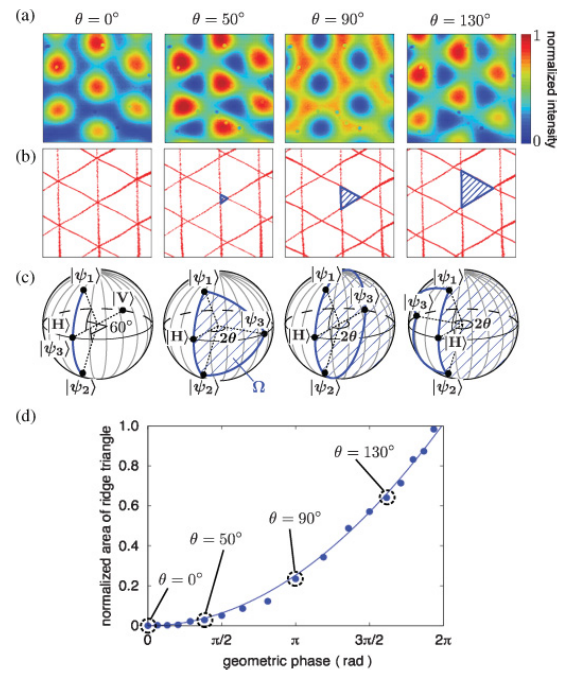
\includegraphics[width=11cm]{paperImages/3}
\par\end{centering}

\protect\caption{Interferogram, data extraction, physical states, prediction and data}
\end{figure}



\section{References}

\url{http://math.stackexchange.com/questions/901819/direct-formula-for-area-of-a-triangle-formed-by-three-lines-given-their-equatio}

\url{http://en.wikipedia.org/wiki/Bloch_sphere}
\end{document}
